\documentclass[12pt]{article}

\usepackage{sbc-template}
\usepackage[brazil,american]{babel}
\usepackage[utf8]{inputenc}

\usepackage{graphicx}
\usepackage{url}
\usepackage{float}
\usepackage{listings}
\usepackage{color}
\setlength{\marginparwidth}{2cm}
\usepackage{todonotes}
\usepackage{algorithmic}
\usepackage{algorithm}
\usepackage{hyperref}
\usepackage{plantuml}

\sloppy


\title{Trabalho Prático\\ 
Cartolitos CF}

%author{Nome do Aluno, Matrícula\\
\author{Élvis Júnior, 24/1038700\\
        Gustavo Alves, 24/1020779\\
        Pedro Marcinoni, 24/1002396\\
        Grupo 1
}

\address{Dep. Ciência da Computação -- Universidade de Brasília (UnB)\\
  CIC0197 - Técnicas de Programação I\\
  \email{elvismirandajr@gmailcom, gusfring.a@gmail.com, pedroextrer@gmail.com}
}

\begin{document}
\maketitle

\selectlanguage{american}
\begin{abstract}
  This document describes the final project of the course "Técnicas de Programação I" at Universidade de Brasília. The project is a desktop application that allows users to manage their fantasy football teams, providing features such as team creation, player selection, and match simulation. The application is built following object-oriented programming principles and utilizes design patterns to ensure maintainability and scalability.
\end{abstract}
\selectlanguage{brazil}

\begin{resumo}
  Este documento descreve o projeto final da disciplina Técnicas de Programação I da Universidade de Brasília. O projeto é uma aplicação desktop que permite aos usuários gerenciar suas equipes de futebol \textit{fantasy}, oferecendo recursos como criação de equipes, seleção de jogadores e simulação de partidas. A aplicação é construída seguindo princípios de programação orientada a objetos e utiliza padrões de design para garantir manutenibilidade e escalabilidade.
\end{resumo}


\section{Descrição do Problema}
\label{sec:descricao}

Como bons brasileiros, quem não gosta de futebol? Foi pensando nisso que a emissora mais famosa do país, a Rede Globe, criou a Cartolitos CF, o novo Fantasy Game do momento, que reflete em tempo real os resultados estatísticos da Copa do Mundo de Clubes, o mais novo fenômeno do futebol. Veja também \cite{wiki:cartola,wiki:fantasy}.

Disponível para computador, o aplicativo permite que os usuários escalem seus times comprando jogadores dos 32 clubes do torneio com “cartoletas” — a moeda virtual do jogo — e pontue de acordo com o desempenho real desses atletas em campo na rodada. Assim, os participantes podem comparar seus resultados com os amigos em uma liga estilo tiro-curto, na qual se considera apenas uma única rodada.

Para colocar esse projeto em prática, a empresa designou três estudantes de Ciência da Computação — Elvis Miranda, Gustavo Alves e Pedro Marcinoni — para desenvolver um programa capaz de auxiliar na logística de gestão de qualquer liga de tiro-curto, servindo depois como base para o funcionamento integral do aplicativo.


\section{Definição das regras de negócio}
\label{sec:regras}

\begin{enumerate}
  \item Função do programa:
        \begin{enumerate}
          \item Cadastrar usuários, clubes, jogadores e equipes de usuários
          \item Simula estatísticas e pontuações conforme regras de negócios
          \item era resultados da liga e rankings
        \end{enumerate}
  \item Identificação: Cada usuário tem ID único, nome, e-mail e senha.
  \item Orçamento: Cada usuário começa com 150 cartoletas.
  \item Escalação:
        \begin{enumerate}
          \item O time do usuário deve ter formação 4-3-3, ou seja, 1 goleiro, 4 defensores, 3 meio-campistas e 3 atacantes.
          \item O time do usuário não pode ter jogadores duplicados.
        \end{enumerate}
  \item Capitão: Cada time deve ter um capitão, que recebe o dobro de pontos.
  \item Estatísticas dos jogadores:
        \begin{enumerate}
          \item Cada jogador possui um preço base e uma nota (overall) que varia de 0 a 100.
          \item Cada confronto (casa/fora) usa as notas de cada jogador para ajustar as probabilidades de contribuir com gols, assistências, desarmes, etc.
        \end{enumerate}
  \item Pontuação:
        \begin{enumerate}
          \item Goleiros:
                \begin{itemize}
                  \item Defesa de pênalti: +7 pontos
                  \item Defesa: +1.5 pontos
                  \item Gol sofrido: -1 ponto
                  \item Não sofrer gol: +5 pontos
                \end{itemize}
          \item Defensores:
                \begin{itemize}
                  \item Desarme: +1.5 pontos
                  \item Falta cometida: -0.5 pontos
                  \item Gol contra: -5 pontos
                  \item Cartão amarelo: -1 pontos
                  \item Cartão vermelho: -3 pontos
                \end{itemize}
          \item Meio-campistas:
                \begin{itemize}
                  \item Assistência: +5 pontos
                  \item Gol: +8 pontos
                  \item Falta cometida: -0.5 pontos
                  \item Desarme: +1.5 pontos
                \end{itemize}
          \item Atacantes:
                \begin{itemize}
                  \item Gol: +8 pontos
                  \item Assistência: +5 pontos
                  \item Finalização: +0.8 pontos
                  \item Falta cometida: -0.5 pontos
                \end{itemize}
        \end{enumerate}
  \item Simulação de partidas: O administrador do programa pode simular partidas entre os times cadastrados, gerando estatísticas e pontuações para cada jogador.
  \item Resultados da liga: O programa deve gerar resultados da liga, mostrando a pontuação total de cada time e o ranking dos usuários.
\end{enumerate}

\section{Diagrama de classes final}
\label{sec:classes}

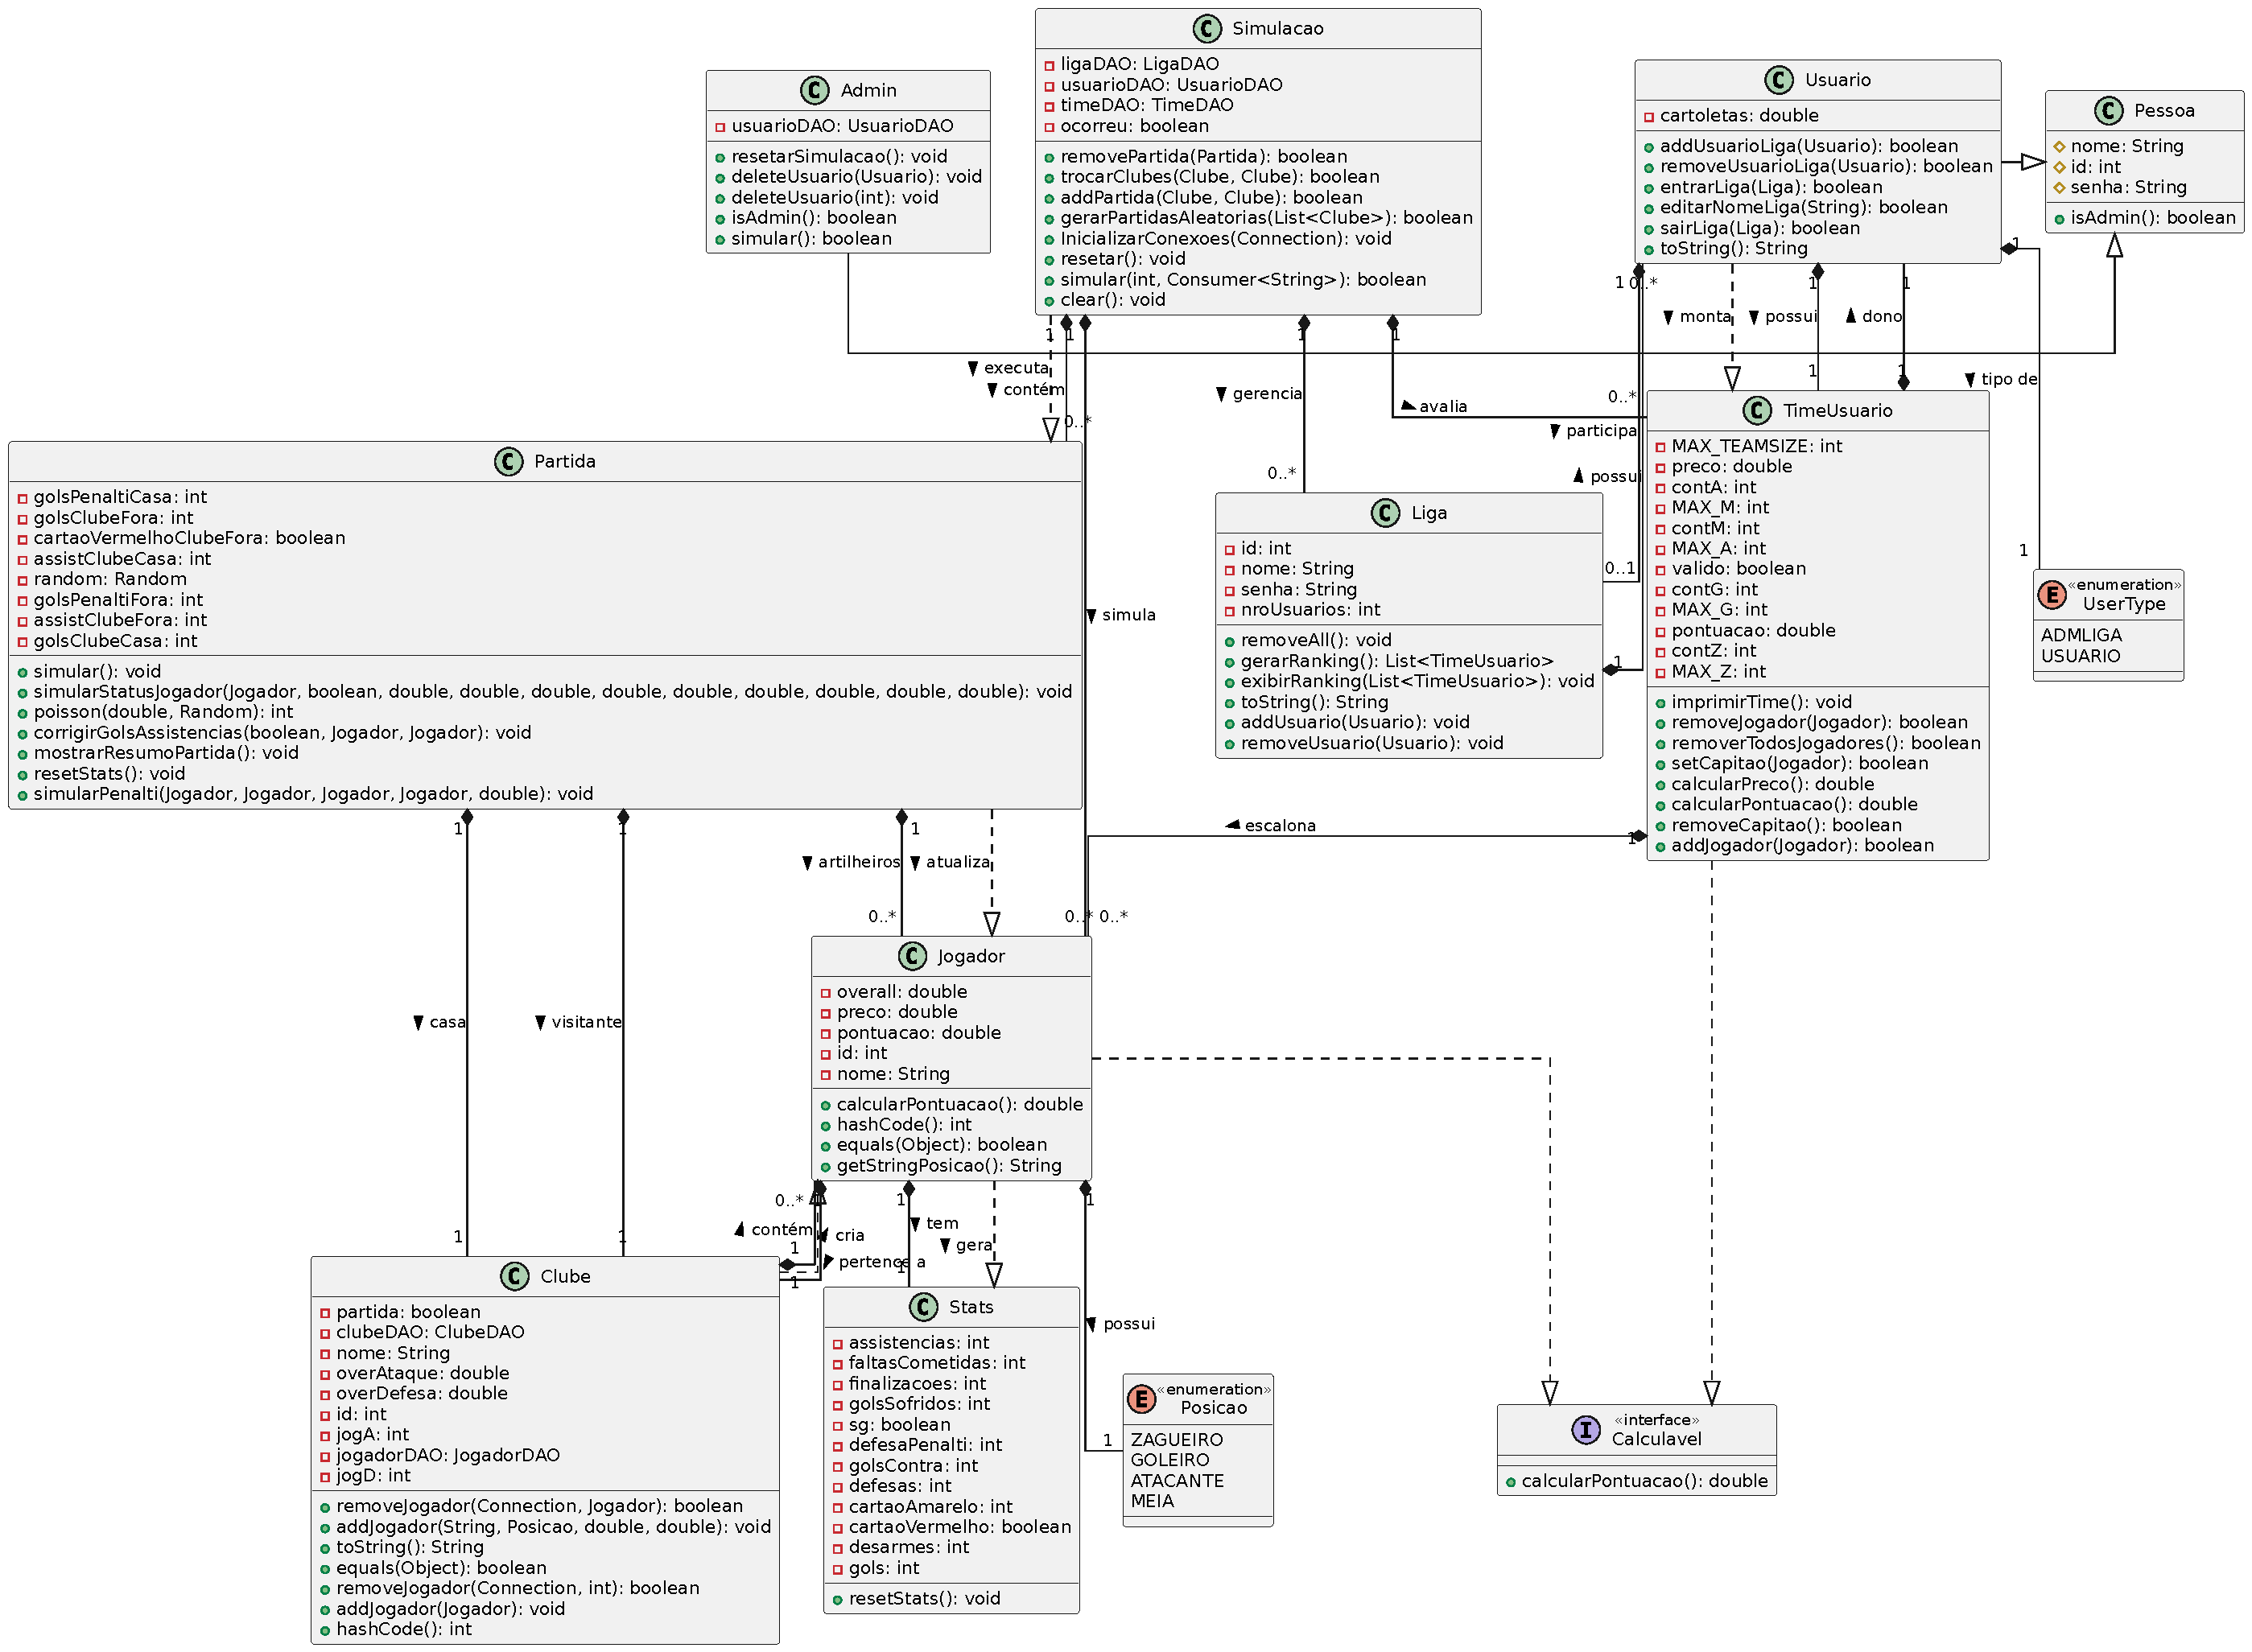
\includegraphics[width=\textwidth]{Diagrama.pdf}

\subsection{Classe abstrata Pessoa}

A classe abstrata \textbf{Pessoa} representa o conceito genérico de uma pessoa dentro do sistema, servindo como base para outras classes mais específicas, como usuários comuns e administradores. Ela define os principais atributos e comportamentos compartilhados por todas as pessoas cadastradas no sistema.

\begin{itemize}
  \item \textbf{Atributos:}
        \begin{itemize}
          \item \texttt{id}: identificador único de cada pessoa.
          \item \texttt{nome}: nome da pessoa.
          \item \texttt{senha}: senha utilizada para autenticação no sistema.
        \end{itemize}
  \item \textbf{Métodos:}
        \begin{itemize}
          \item \texttt{getId()}: retorna o identificador da pessoa.
          \item \texttt{getNome()} e \texttt{setNome(String nome)}: obtêm e alteram o nome da pessoa.
          \item \texttt{getSenha()} e \texttt{setSenha(String senha)}: obtêm e alteram a senha da pessoa.
          \item \texttt{isAdmin()}: indica se a pessoa é um administrador. Por padrão, retorna \texttt{false}, mas pode ser sobrescrito em subclasses.
        \end{itemize}
\end{itemize}

Dessa forma, a classe \textbf{Pessoa} garante a reutilização de código e facilita a manutenção, permitindo que funcionalidades comuns sejam implementadas uma única vez e herdadas pelas demais classes do sistema.

\subsubsection{Sublasse Usuario}

A subclasse \textbf{Usuario} representa um usuário do sistema, sendo uma especialização da classe abstrata \texttt{Pessoa}. Ela adiciona atributos e comportamentos específicos relacionados à participação do usuário em ligas e à administração dessas ligas.

\begin{itemize}
  \item \textbf{Atributos principais:}
        \begin{itemize}
          \item \texttt{cartoletas}: representa o saldo virtual do usuário, utilizado para comprar jogadores.
          \item \texttt{tipo}: indica o tipo do usuário, podendo ser comum ou administrador de liga.
          \item \texttt{timeUsuario}: armazena o time montado pelo usuário.
          \item \texttt{liga}: referência à liga da qual o usuário faz parte.
        \end{itemize}
  \item \textbf{Métodos principais:}
        \begin{itemize}
          \item \texttt{editarNomeLiga(String novoNome)}: permite ao administrador de liga alterar o nome da liga.
          \item \texttt{addUsuarioLiga(Usuario usuario)}: permite ao administrador adicionar um novo usuário à liga.
          \item \texttt{removeUsuarioLiga(Usuario usuario)}: permite ao administrador remover um usuário da liga.
          \item \texttt{entrarLiga(Liga liga)}: permite ao usuário entrar em uma liga, caso ainda não participe de nenhuma.
          \item \texttt{sairLiga(Liga liga)}: permite ao usuário sair da liga atual.
          \item \texttt{toString()}: retorna uma representação textual do usuário, exibindo seu ID e nome.
        \end{itemize}
\end{itemize}

Esses métodos garantem as principais operações de gerenciamento de ligas e participação dos usuários, respeitando as regras de negócio do sistema.

\subsubsection{Sublasse Admin}

A subclasse \textbf{Admin} representa o administrador do sistema, sendo uma especialização da classe abstrata \texttt{Pessoa}. Ela é responsável por operações administrativas, como gerenciamento de usuários e simulação de partidas.

\begin{itemize}
  \item \textbf{Atributos principais:}
        \begin{itemize}
          \item \texttt{usuarioDAO}: objeto responsável pelo acesso e manipulação dos dados dos usuários no banco de dados.
        \end{itemize}
  \item \textbf{Métodos principais:}
        \begin{itemize}
          \item \texttt{Admin(int id, String nome, String senha, Connection conn)}: construtor que inicializa o administrador e o objeto de acesso a dados.
          \item \texttt{simular()}: executa a simulação das partidas do sistema.
          \item \texttt{resetarSimulacao()}: reseta os dados da simulação realizada.
          \item \texttt{deleteUsuario(Usuario usuario)}: remove um usuário do sistema a partir de um objeto \texttt{Usuario}.
          \item \texttt{deleteUsuario(int id)}: remove um usuário do sistema a partir do seu identificador.
          \item \texttt{isAdmin()}: sobrescreve o método da classe \texttt{Pessoa} para indicar que esta instância é de um administrador.
        \end{itemize}
\end{itemize}

Esses métodos permitem ao administrador controlar usuários e simulações, garantindo a manutenção e o funcionamento correto do sistema.

\subsection{Classe TimeUsuario}

A classe \textbf{TimeUsuario} representa o time montado por um usuário, sendo responsável por gerenciar a escalação, o capitão, o cálculo de pontuação e o controle de validade do time para simulação.

\begin{itemize}
  \item \textbf{Atributos principais:}
        \begin{itemize}
          \item \texttt{usuario}: referência ao usuário dono do time.
          \item \texttt{jogadores}: conjunto de jogadores escalados no time.
          \item \texttt{pontuacao}: pontuação total do time após a simulação.
          \item \texttt{preco}: valor total do time, somando o preço de todos os jogadores.
          \item \texttt{capitao}: jogador escolhido como capitão, que tem sua pontuação dobrada.
          \item \texttt{valido}: indica se a escalação está válida para simulação (time completo e capitão definido).
          \item \texttt{contG}, \texttt{contZ}, \texttt{contM}, \texttt{contA}: contadores de jogadores por posição (goleiro, zagueiro, meia e atacante).
        \end{itemize}
  \item \textbf{Métodos principais:}
        \begin{itemize}
          \item \texttt{TimeUsuario(Usuario usuario)}: construtor que inicializa um time vazio para o usuário.
          \item \texttt{TimeUsuario(Usuario usuario, Set<Jogador> jogadores, Jogador jogcapitao)}: construtor que inicializa o time já com jogadores e capitão.
          \item \texttt{calcularPontuacao()}: calcula a pontuação total do time, considerando o capitão.
          \item \texttt{calcularPreco()}: calcula o preço total do time.
          \item \texttt{addJogador(Jogador jogador)}: adiciona um jogador ao time, respeitando as regras de quantidade e orçamento.
          \item \texttt{removeJogador(Jogador jogador)}: remove um jogador do time.
          \item \texttt{setCapitao(Jogador jogador)}: define o capitão do time, caso o jogador esteja escalado.
          \item \texttt{removeCapitao()}: remove o capitão do time.
          \item \texttt{removerTodosJogadores()}: remove todos os jogadores do time.
          \item \texttt{imprimirTime()}: imprime no console as informações do time, incluindo jogadores, pontuação e capitão.
          \item \texttt{getGoleiro()}, \texttt{getZagueiros()}, \texttt{getMeias()}, \texttt{getAtacantes()}: retornam os jogadores do time por posição.
          \item \texttt{getTodosOsEscalados()}: retorna todos os jogadores do time, organizados por posição.
        \end{itemize}
\end{itemize}

Esses métodos permitem ao usuário montar, visualizar e gerenciar seu time, garantindo que a escalação siga as regras do sistema e esteja pronta para a simulação das partidas.

\subsection{Classe Liga}

A classe \textbf{Liga} representa uma liga do sistema, permitindo o agrupamento de usuários para competições e gerenciamento de rankings.

\begin{itemize}
  \item \textbf{Atributos principais:}
        \begin{itemize}
          \item \texttt{id}: identificador único da liga.
          \item \texttt{nroUsuarios}: quantidade de usuários participantes da liga.
          \item \texttt{nome}: nome da liga.
          \item \texttt{senha}: senha de acesso à liga.
          \item \texttt{usuarios}: lista de usuários que participam da liga.
        \end{itemize}
  \item \textbf{Métodos principais:}
        \begin{itemize}
          \item \texttt{Liga(int id, String nome, String senha)}: construtor que inicializa a liga com identificador, nome e senha.
          \item \texttt{removeAll()}: remove todos os usuários da liga.
          \item \texttt{addUsuario(Usuario usuario)}: adiciona um usuário à liga e incrementa o número de participantes.
          \item \texttt{removeUsuario(Usuario usuario)}: remove um usuário da liga e decrementa o número de participantes.
          \item \texttt{gerarRanking()}: gera e retorna uma lista dos times dos usuários, ordenada pela pontuação (ranking da liga).
          \item \texttt{exibirRanking(List<TimeUsuario> times)}: exibe no console o ranking dos times da liga.
          \item \texttt{toString()}: retorna uma representação textual da liga, mostrando seu nome.
        \end{itemize}
\end{itemize}

Esses métodos permitem o gerenciamento dos participantes e o acompanhamento do desempenho dos times dentro de uma liga, proporcionando a competição entre os usuários.

\subsection{Classe Simulacao}

A classe \textbf{Simulacao} é responsável por gerenciar o processo de simulação das partidas entre clubes, além de controlar o estado das simulações e o relacionamento com as ligas e usuários do sistema.

\begin{itemize}
  \item \textbf{Atributos principais:}
        \begin{itemize}
          \item \texttt{ocorreu}: indica se a simulação já foi realizada.
          \item \texttt{partidas}: conjunto de partidas que serão simuladas.
          \item \texttt{ligaDAO}: objeto responsável pelo acesso e manipulação dos dados das ligas no banco de dados.
          \item \texttt{usuarioDAO}: objeto responsável pelo acesso e manipulação dos dados dos usuários no banco de dados.
        \end{itemize}
  \item \textbf{Métodos principais:}
        \begin{itemize}
          \item \texttt{InicializarConexoes(Connection conn)}: inicializa os objetos de acesso a dados com a conexão ao banco.
          \item \texttt{gerarPartidasAleatorias(List<Clube> clubes)}: sorteia clubes em partidas aleatórias, garantindo que todos participem.
          \item \texttt{addPartida(Clube clubeCasa, Clube clubeFora)}: adiciona uma partida entre dois clubes, se ambos ainda não estiverem em outra partida.
          \item \texttt{simular()}: executa a simulação das partidas e calcula a pontuação dos jogadores e times das ligas.
          \item \texttt{resetar()}: reseta o estado da simulação, restaurando os dados dos jogadores e times.
          \item \texttt{trocarClubes(Clube clube1, Clube clube2)}: troca clubes entre partidas diferentes.
          \item \texttt{clear()}: limpa todas as partidas da simulação e libera os clubes para novas partidas.
        \end{itemize}
\end{itemize}

Esses métodos permitem o controle completo do ciclo de simulação das partidas, desde a geração dos confrontos até o cálculo e a reinicialização dos resultados.

\subsection{Interface Simulavel}

A interface \textbf{Simulavel} define um contrato para as classes que desejam implementar a funcionalidade de simulação no sistema. Ela garante que qualquer classe que a implemente possua o método necessário para realizar uma simulação.

\begin{itemize}
  \item \textbf{Métodos principais:}
        \begin{itemize}
          \item \texttt{simular()}: método abstrato que deve ser implementado pelas classes concretas, responsável por executar a lógica de simulação específica de cada classe.
        \end{itemize}
\end{itemize}

Dessa forma, a interface \textbf{Simulavel} promove a padronização e a reutilização de código, permitindo que diferentes componentes do sistema possam ser simulados de maneira uniforme.

\subsubsection{Classe Partida}

A classe \textbf{Partida}, implementação da interface \textbf{Simulavel} representa um confronto entre dois clubes no sistema, sendo responsável por simular o jogo, calcular estatísticas dos jogadores e armazenar os principais eventos da partida.

\begin{itemize}
  \item \textbf{Atributos principais:}
        \begin{itemize}
          \item \texttt{clubeCasa}, \texttt{clubeFora}: referências aos clubes que disputam a partida.
          \item \texttt{golsClubeCasa}, \texttt{golsClubeFora}: quantidade de gols marcados por cada clube.
          \item \texttt{assistClubeCasa}, \texttt{assistClubeFora}: quantidade de assistências de cada clube.
          \item \texttt{golsPenaltiCasa}, \texttt{golsPenaltiFora}: quantidade de gols de pênalti de cada clube.
          \item \texttt{jogadoresGolCasa}, \texttt{jogadoresGolFora}: listas de jogadores que marcaram gols por cada clube.
          \item \texttt{jogadoresAssistenciaCasa}, \texttt{jogadoresAssistenciaFora}: listas de jogadores que deram assistências por cada clube.
          \item \texttt{cartaoVermelhoClubeCasa}, \texttt{cartaoVermelhoClubeFora}: indicam se algum jogador do clube recebeu cartão vermelho.
          \item \texttt{random}: objeto para geração de números aleatórios, utilizado na simulação dos eventos da partida.
        \end{itemize}
  \item \textbf{Métodos principais:}
        \begin{itemize}
          \item \texttt{Partida(Clube clubeCasa, Clube clubeFora)}: construtor que inicializa uma partida entre dois clubes.
          \item \texttt{simular()}: executa toda a lógica de simulação da partida, gerando estatísticas para os jogadores e clubes.
          \item \texttt{simularStatusJogador(...)}: simula os eventos individuais de cada jogador (gols, assistências, desarmes, faltas, cartões, etc.).
          \item \texttt{simularPenalti(...)}: simula a ocorrência de pênaltis, gols e defesas de pênalti na partida.
          \item \texttt{corrigirGolsAssistencias(...)}: ajusta a relação entre gols e assistências para garantir consistência nos dados da partida.
          \item \texttt{resetStats()}: reseta todas as estatísticas da partida e dos jogadores envolvidos, preparando para uma nova simulação.
          \item \texttt{mostrarResumoPartida()}: exibe no console um resumo detalhado dos principais eventos e estatísticas da partida.
          \item \texttt{poisson(double lambda, Random random)}: calcula um valor aleatório baseado na distribuição de Poisson, utilizado para simular eventos como gols e assistências.
          \item \texttt{calcularBonusClube(boolean timeCasa)}: calcula bônus de desempenho para o clube, considerando fatores como mando de campo e cartões vermelhos.
          \item \texttt{getAllJogadores()}: retorna uma lista com todos os jogadores participantes da partida.
        \end{itemize}
\end{itemize}

Esses métodos e atributos permitem simular partidas de forma realista, atribuindo estatísticas individuais aos jogadores e resultados aos clubes, além de possibilitar o acompanhamento detalhado dos eventos ocorridos durante o jogo.

\subsection{Classe Jogador}

A classe \textbf{Jogador} representa um atleta disponível para ser escalado nos times dos usuários, armazenando informações essenciais para a simulação e pontuação.

\begin{itemize}
  \item \textbf{Atributos principais:}
        \begin{itemize}
          \item \texttt{id}: identificador único do jogador.
          \item \texttt{nome}: nome do jogador.
          \item \texttt{posicao}: posição em que o jogador atua (goleiro, zagueiro, meia ou atacante).
          \item \texttt{clube}: referência ao clube ao qual o jogador pertence.
          \item \texttt{preco}: valor do jogador em cartoletas.
          \item \texttt{overall}: nota geral do jogador, utilizada para simulação de desempenho.
          \item \texttt{pontuacao}: pontuação total do jogador após a simulação.
          \item \texttt{stats}: objeto que armazena as estatísticas detalhadas do jogador na partida.
        \end{itemize}
  \item \textbf{Métodos principais:}
        \begin{itemize}
          \item \texttt{Jogador(int id, String nome, Posicao posicao, Clube clube, double preco, double overall)}: construtor que inicializa o jogador com seus dados básicos.
          \item \texttt{getStringPosicao()}: retorna a posição do jogador em formato textual.
          \item \texttt{calcularPontuacao()}: calcula e atualiza a pontuação do jogador com base em suas estatísticas e regras de pontuação do sistema.
          \item \texttt{equals(Object obj)} e \texttt{hashCode()}: métodos sobrescritos para garantir a correta comparação e uso do jogador em coleções.
        \end{itemize}
\end{itemize}

Esses métodos e atributos permitem representar, identificar e calcular o desempenho de cada jogador, sendo fundamentais para a lógica de escalação e simulação das partidas.

\subsection{Classe Stats}

A classe \textbf{Stats} representa as estatísticas detalhadas de desempenho de um jogador em uma partida, armazenando informações essenciais para o cálculo da pontuação individual.

\begin{itemize}
  \item \textbf{Atributos principais:}
        \begin{itemize}
          \item \texttt{desarmes}: quantidade de desarmes realizados pelo jogador.
          \item \texttt{gols}: quantidade de gols marcados.
          \item \texttt{assistencias}: quantidade de assistências realizadas.
          \item \texttt{sg}: indica se o jogador terminou a partida sem sofrer gols (aplicável a goleiros e zagueiros).
          \item \texttt{finalizacoes}: número de finalizações feitas.
          \item \texttt{defesas}: número de defesas realizadas (goleiros).
          \item \texttt{defesaPenalti}: número de defesas de pênalti.
          \item \texttt{golsContra}: quantidade de gols contra marcados.
          \item \texttt{cartaoVermelho}: indica se o jogador recebeu cartão vermelho.
          \item \texttt{golsSofridos}: quantidade de gols sofridos (goleiros e zagueiros).
          \item \texttt{cartaoAmarelo}: quantidade de cartões amarelos recebidos.
          \item \texttt{faltasCometidas}: número de faltas cometidas.
          \item \texttt{posicao}: posição do jogador na partida.
        \end{itemize}
  \item \textbf{Métodos principais:}
        \begin{itemize}
          \item \texttt{resetStats()}: reseta todas as estatísticas do jogador para os valores iniciais, preparando para uma nova simulação.
          \item \texttt{forEach(Consumer<? super Map.Entry<String, Integer>> action)}: percorre todas as estatísticas, permitindo executar uma ação para cada uma delas (útil para exibição ou processamento).
        \end{itemize}
\end{itemize}

Esses métodos e atributos permitem registrar, manipular e exibir as estatísticas individuais dos jogadores, sendo fundamentais para o cálculo da pontuação e para a análise de desempenho nas partidas simuladas.

\subsection{Classe Clube}

A classe \textbf{Clube} representa um clube de futebol no sistema, armazenando informações sobre seus jogadores, desempenho médio e integração com o banco de dados.

\begin{itemize}
  \item \textbf{Atributos principais:}
        \begin{itemize}
          \item \texttt{id}: identificador único do clube.
          \item \texttt{nome}: nome do clube.
          \item \texttt{overAtaque}: média aritmética do overall dos jogadores de ataque do clube.
          \item \texttt{overDefesa}: média aritmética do overall dos jogadores de defesa do clube.
          \item \texttt{jogadores}: conjunto de jogadores pertencentes ao clube.
          \item \texttt{jogA}, \texttt{jogD}: quantidade de jogadores de ataque e defesa, respectivamente.
          \item \texttt{partida}: indica se o clube já está escalado para uma partida.
          \item \texttt{clubeDAO}, \texttt{jogadorDAO}: objetos responsáveis pelo acesso e manipulação dos dados do clube e dos jogadores no banco de dados.
        \end{itemize}
  \item \textbf{Métodos principais:}
        \begin{itemize}
          \item \texttt{Clube(...)}: construtores que inicializam o clube, podendo inserir ou recuperar dados do banco de dados.
          \item \texttt{addJogador(String nomeJogador, Posicao posicao, double preco, double overall)}: adiciona um novo jogador ao clube e ao banco de dados.
          \item \texttt{addJogador(Jogador jogador)}: adiciona ao clube um jogador já existente no banco de dados.
          \item \texttt{removeJogador(Connection conn, Jogador jogador)}: remove um jogador do clube e do banco de dados, se a simulação ainda não ocorreu.
          \item \texttt{removeJogadorById(Connection conn, int idJogador)}: remove um jogador pelo ID, tanto do clube quanto do banco de dados.
          \item \texttt{recalcOverAtaqueAdd/Sub(double overall)} e \texttt{recalcOverDefesaAdd/Sub(double overall)}: recalculam a média de overall de ataque ou defesa ao adicionar ou remover jogadores.
          \item \texttt{isAtaque(Posicao posicao)} e \texttt{isDefesa(Posicao posicao)}: verificam se uma posição é considerada de ataque ou defesa.
          \item \texttt{toString()}: retorna uma representação textual do clube.
        \end{itemize}
\end{itemize}

Esses métodos e atributos permitem o gerenciamento completo dos clubes, incluindo a manutenção dos jogadores, atualização das médias de desempenho e integração com o banco de



\section{Telas}
\label{sec:telas}

\subsection{Telas Iniciais}
\label{sec:telas_iniciais}

O programa possui dois fluxos principais: o fluxo do usuário e o fluxo do administrador. Cada um possui telas específicas para suas funcionalidades.

\subsection{Fluxo do usuário}
\label{sec:fluxo_usuario}
\subsubsection{Menu Principal}
\label{sec:menu_principal}
\subsubsection{Ligas}
\label{sec:ligasUsr}


\section{Conclusão}
\label{sec:conclusao}

Colocar aqui a conclusão do projeto. O que foi aprendido? O que poderia ser melhorado? Quais as dificuldades encontradas? Quais os próximos passos?

\bibliographystyle{sbc}
\bibliography{relatorio}  %Aqui é a definição do arquivo .bib a ser usado pelas referências

% Adicione as referências ausentes diretamente aqui para evitar erro de citação
\begin{thebibliography}{99}
  \bibitem{wiki:cartola}
  Cartola FC. Disponível em: \url{https://pt.wikipedia.org/wiki/Cartola_FC}. Acesso em: 10 jun. 2024.

  \bibitem{wiki:fantasy}
  Fantasy Sports. Disponível em: \url{https://en.wikipedia.org/wiki/Fantasy_sport}. Acesso em: 10 jun. 2024.
\end{thebibliography}


\end{document}
